\documentclass[12pt,oneside,a4paper]{book}

\input{./AuxFiles/Packages}

\title{Decentralized LoRa Mesh Network for Wearable Public Safety using Blockchain and Federated Learning}
\subCode{IDP}
\Department[AI\&ML]{Artificial Intelligence and Machine Learning}
\academicYear{2025-26}

\IDPProject

\MastersIn[B.E]{Bachelor of Engineering}
\pgProgramName{Artificial Intelligence and Machine Learning}

\stuNameA{Kunal Rathod}
\stuUSNA{1RV23ME060}
\stuNameB{Abhinav Potharaju}
\stuUSNB{1RV23AI135}
\stuNameC{Akshad Jagdale}
\stuUSNC{1RV23ME017}
\stuNameD{Ibrahim Bagwan}
\stuUSND{1RV24AI404}

\guideNameA{Prof. Saraswathi Govind Datar}
\guideDesignationA{Professor}
\guideDeptA[CSE]{Computer Science and Engineering}
\guideOrgA{RV College of Engineering}

\panelMemberNameA{Prof. Savithri Kulkarni}
\panelMemberDesigA{Assistant Professor}
\panelMemberDeptA[CSE]{Computer Science and Engineering}
\panelMemberNameB{Dr. Shanta Rangaswamy}
\panelMemberDesigB{Professor \& Head}
\panelMemberDeptB[CSE]{Computer Science and Engineering}

\projectCoOrdNameA{Dr. Prapulla S B}
\projectCoOrdDesigA{Associate Professor}
\projectCoOrdDeptA[CSE]{Computer Science and Engineering}

\HOD{Dr. Shanta Rangaswamy}
\Principal{Dr. K. N. Subramanya}
\DeanAcademics{Dr. M.V. Renukadevi}
\VicePrincipal{Dr. Geetha K S}

\QRurl{}

\newglossary[sym]{symbolList}{sym1}{sym2}{List of Symbols}
\makeglossaries
\loadglsentries{./AuxFiles/Glossaries}
\renewcommand{\glspostdescription}{}

\usepackage[backend=bibtex,style=ieee]{biblatex}
\addbibresource{./AuxFiles/ProjectBib.bib}

\usepackage{background}
\backgroundsetup{scale=1, angle=0, firstpage = false, opacity=0.5, contents={
\begin{tikzpicture}[remember picture, overlay]
\node at ([yshift=0pt, xshift=0pt]current page.center){
\includegraphics[width=0.6\textwidth]{Figures/RVlogoVecW}};
\end{tikzpicture}
}}

\definecolor{coverGreen}{RGB}{161,214,165}

\begin{document}
\NoBgThispage
\pagecolor{coverGreen}
\maketitle
\pagecolor{white}
\newpage
\ifDrf
\else
\begin{spacing}{1.5}
\input{./CoverPages/Certificate}

\newpage
\input{./CoverPages/Declaration}

\newpage
\input{./CoverPages/Ack}

\newpage
\pagenumbering{roman}

\chapter*{Abstract}
\addcontentsline{toc}{chapter}{Abstract}\vspace{-1cm}
%Border
\begin{tikzpicture}[remember picture, overlay]
  \draw[line width = 4pt] ($(current page.north west) + (0.75in,-0.75in)$) rectangle ($(current page.south east) + (-0.75in,0.75in)$);
\end{tikzpicture}

Dysarthria is a motor speech disorder caused by neurological conditions such as ALS, cerebral palsy, Parkinson’s disease, and stroke. It affects speech muscles, resulting in slurred or slow speech that can be difficult to understand. Severity varies widely and can significantly impact communication. Traditional methods of assessing and treating dysarthria often involve in-person evaluations and therapy sessions, which can be time-consuming and may not be accessible to all patients. Globally, millions of people suffer from speech impairments, yet most speech technologies are trained only on normal speech. Highlighting the need for more efficient, technology-driven solutions. This report presents a novel system that leverages advanced techniques to improve accessibility and communication for individuals with dysarthria.

The objectives of this work is to generate synthetic dysarthric speech using Text-to-Speech (TTS) and GAN-based voice conversion techniques and to develop a post-ASR semantic correction layer utilizing large language models for improved transcription accuracy which enhances system robustness through noise augmentation and advanced acoustic feature extraction methods. We finally wish to integrate a Personal Knowledge Graph to support contextual speech disambiguation

We were able to achieve a significant improvement in the accuracy of dysarthric speech recognition by implementing a novel architecture that combines advanced acoustic feature extraction methods with a post-ASR semantic correction in the layers of whispher model by openai. The system was trained and evaluated using a dataset of dysarthric speech samples, and we observed a sub 20\% WER in transcription accuracy which is better compared to previous approaches. The integration of a Personal Knowledge Graph for contextual speech disambiguation further enhanced the system's performance, particularly in noisy environments.  
\pagebreak

\end{spacing}
\newpage
\pagestyle{fplain}
\begin{spacing}{1.5}
\tableofcontents	
\end{spacing}
\newpage
\begin{spacing}{1.5}
\cleardoublepage
\addcontentsline{toc}{chapter}{List of Figures}
\listoffigures	
\end{spacing}
\newpage
\begin{spacing}{1.5}
\cleardoublepage
\addcontentsline{toc}{chapter}{List of Tables}
\listoftables	
\end{spacing}

\printglossary[type=\acronymtype, title= Abbreviations, toctitle=Abbreviations]
\printglossary[type=symbolList, title= List of Symbols, toctitle=List of Symbols]
\fi
\mainmatter
\pagestyle{mplain}
\glsresetall
\begin{spacing}{1.5}

\chapter{Introduction}

\section{Introduction}

First responders operating in infrastructure-denied environments—burning structures, collapsed buildings, remote terrain, or contested urban zones—depend on communication and monitoring systems designed for normal conditions. When those conditions collapse, so do the systems. The 9/11 World Trade Center communications failure, in which 343 firefighters perished partly because their radios were incompatible with police channels \cite{NIST_9_11_comms}, and Hurricane Katrina in 2005, where the loss of cell towers paralysed coordinated rescue for 60,000 stranded survivors \cite{AFCEA_Katrina_comms}, illustrate a persistent architectural failure: centralised, infrastructure-dependent designs are most vulnerable precisely when they are most needed.

This project proposes a fundamentally different architecture. Each responder carries a self-contained wearable node built on the ESP32-C3 microcontroller and Semtech SX1276 LoRa transceiver that participates in a peer-to-peer mesh network requiring no pre-existing infrastructure. Every node runs a lightweight SHA-256 Proof-of-Authority (PoA) blockchain that creates a cryptographically verifiable, tamper-evident log of sensor events. A Federated Averaging (FedAvg) layer trains an on-device logistic regression anomaly detector collaboratively across all nodes by exchanging gradient weight vectors rather than raw biometric data, protecting physiological privacy while enabling collective learning.

The technical novelty lies in the co-design of all three layers—LoRa mesh, on-device blockchain, and over-the-air federated learning—on commodity microcontroller hardware under strict power, memory (320~KB SRAM), and bandwidth constraints (37.5~kbps maximum physical-layer throughput). The system is validated against a hybrid testbed combining physical ESP32-C3 nodes with software-simulated virtual nodes connected via an MQTT bridge, enabling performance characterisation at network scales impractical to instrument purely in hardware.

\section{Problem Statement}

The fundamental problem is the absence of a low-cost, infrastructure-independent, tamper-resistant wearable network that can provide real-time physiological monitoring, secure data logging, and distributed anomaly detection for first-responder teams where conventional communications infrastructure is unavailable.

Three distinct gaps drive this work:

\textbf{(1) Infrastructure dependency.} Existing wearable platforms conforming to NIST IR 8235 \cite{NIST_IR_8235} rely on cellular data or proprietary radio protocols requiring fixed base stations. When infrastructure is destroyed—exactly when monitoring is most critical—monitoring capability is lost.

\textbf{(2) Data integrity.} Sensor data stored on centralised servers is vulnerable to corruption and tampering. In forensic contexts (determining whether a responder's vitals were safe before entering a collapse zone), integrity must be provable without relying on any single custodian. Existing blockchain implementations target high-bandwidth, unconstrained environments; running one on a microcontroller with 320~KB SRAM over a 37.5~kbps radio requires a purpose-designed approach \cite{Semtech_SX1276_datasheet}.

\textbf{(3) Biometric privacy.} Heart rate, SpO2, and fall events are sensitive health data. Centralising them creates a single point of failure for privacy. Federated Learning ensures raw sensor readings never leave the node, but transmitting weight vectors over the low-bandwidth, variable-latency LoRa channel introduces engineering constraints that existing WiFi-centric FL frameworks do not address.

\section{Motivation}

The International Labour Organization estimates 2.3 million occupational fatalities annually, with emergency workers disproportionately represented \cite{ILO_safety_stats}. The NFPA reported 136 on-duty firefighter deaths in the United States in 2021 alone \cite{NFPA_2021_firefighter}; post-incident reviews consistently cite delayed physiological awareness as a contributing factor. Commercial PASS devices detect motion cessation and emit an audible alarm but provide no physiological data, no network communication, and no position fix \cite{IEEE_PST_wearables}.

Three concurrent technology developments now make the proposed architecture feasible. First, the SX1276 LoRa transceiver achieves link budgets exceeding 155~dB with sub-100~mW power, enabling reliable links at 200--1000~m in urban and forested environments \cite{Semtech_SX1276_datasheet}. Second, peer-to-peer LoRa mesh has been demonstrated for mountain rescue and industrial safety without any gateway dependency \cite{LoRa_mesh_rescue_2024}. Third, the ESP32-C3 executes SHA-256 via mbedTLS in under 2~ms per block, making on-device blockchain viable within a 5-second sensor reporting cycle.

Existing alternatives are inadequate. FirstNet, the US public safety LTE network, loses coverage when cell towers are destroyed \cite{Preprints_FirstNet_5G_review}—as demonstrated in the 2019--2020 Australian bushfires where large areas lost all cellular connectivity for days. Iridium and Globalstar satellite options carry prohibitive per-device cost and latency. P25 and TETRA land mobile radio systems do not carry physiological sensor data or provide cryptographic data integrity. The FL motivation is similarly specific: centralised aggregation of health data is vulnerable to gradient inversion attacks even when data is encrypted in transit \cite{FL_privacy_threats_survey_2024}, while FedAvg with differential privacy provides a rigorous bound on per-individual information leakage \cite{FL_DP_McMahan2018}.

\section{Objectives}

\begin{enumerate}
    \item Integrate MPU6050 IMU, MAX30102 PPG sensor, and SX1276 LoRa transceiver on the ESP32-C3 for concurrent fall detection, heart rate, and SpO2 measurement.
    \item Implement SHA-256 PoA blockchain directly on the ESP32-C3 within the 320~KB SRAM constraint.
    \item Establish reliable bidirectional LoRa P2P communication between nodes with per-block hash verification.
    \item Implement FedAvg with Gaussian DP noise over LoRa and demonstrate weight convergence in a bounded number of rounds.
    \item Implement two-phase fall detection and SpO2/HR anomaly alerting with blockchain-logged, LoRa-propagated alert blocks.
    \item Develop a Python simulation (Gudmundson channel model, blockchain, FL) for up to 20 nodes and validate against hardware measurements via MQTT bridge.
\end{enumerate}

\section{Brief Methodology of the Project}

The project follows a milestone-driven methodology: five software simulation milestones (M1--M5) completed prior to hardware procurement, followed by six hardware milestones (M6--M11) building toward full system integration.

\textbf{Simulation phase (M1--M5):} M1 models the SX1276 physical layer with Gudmundson log-normal shadowing to replicate empirical PDR curves. M2 implements a Python SHA-256 hash chain providing ground-truth hashes for firmware verification. M3 processes UCI HAR accelerometer data \cite{UCI_HAR_dataset} for fall detection algorithm development. M4 implements FedAvg with Gaussian DP noise, demonstrating L2-norm convergence across simulated nodes. M5 exercises the full system at 5, 10, and 20 nodes, characterising blockchain propagation latency and FL convergence rate as a function of network size.

\textbf{Hardware phase (M6--M11):} M6 verifies sensor initialisation and valid readings. M7 establishes bidirectional LoRa block exchange with SHA-256 hash verification. M8 exercises multi-block hash chain and prevHash linkage against the Python simulation. M9 implements FedAvg weight exchange on hardware with convergence demonstration. M10 tests the full operational loop including a 10-minute soak test for heap stability. M11 connects physical nodes to the Python simulation mesh via USB-serial JSON bridge and Mosquitto MQTT, verifying three-way chain hash agreement.

\section{Key Contributions}

\begin{itemize}
\item First simultaneous co-integration of SHA-256 PoA blockchain and FedAvg over a LoRa P2P radio on a commodity ESP32-C3 (320~KB SRAM).
\item Airtime-aware TDMA-scheduled FL protocol accounting for the 1.8-second channel occupancy of a 124-byte LoRa block at SF10/BW125.
\item Hybrid MQTT testbed enabling physical ESP32 nodes and Python-simulated virtual nodes to participate in the same mesh as first-class peers.
\end{itemize}

The remainder of this report is organised as follows: Chapter~2 surveys the literature and theoretical foundations; Chapter~3 presents system design; Chapter~4 covers implementation; Chapter~5 reports results; Chapter~6 concludes.

\chapter{Literature Review and Fundamentals}

This chapter surveys the theoretical foundations and state of the art across the five domains underlying this project: LoRa communication, mesh networking, blockchain data integrity, federated learning, and wearable physiological sensing.

% =========================================================
\section{LoRa Physical Layer}

LoRa (Long Range) uses \textbf{Chirp Spread Spectrum (CSS)} modulation, developed by Semtech, in which each symbol is a linearly swept chirp across bandwidth $B$. The processing gain $PG = 10\log_{10}(2^{SF})$~dB allows the receiver to detect signals several dB below the noise floor, and signals at different spreading factors are mutually orthogonal \cite{Semtech2019, Augustin2016}. Three parameters govern performance:

\begin{table}[h]
\centering
\caption{LoRa air-interface configurations and resulting characteristics}
\label{tab:lora_params}
\renewcommand{\arraystretch}{1.2}
\begin{tabular}{ccccc}
\hline
\textbf{SF} & \textbf{BW (kHz)} & \textbf{CR} & \textbf{Bit Rate (bps)} & \textbf{Sensitivity (dBm)} \\
\hline
7  & 125 & 4/5 & 5469 & $-123$ \\
9  & 125 & 4/5 & 1758 & $-129$ \\
10 & 125 & 4/8 & 610  & $-132$ \\
12 & 125 & 4/8 & 183  & $-137$ \\
\hline
\end{tabular}
\end{table}

This project uses SF10/BW125/CR4-8, giving $-132$~dBm sensitivity and a link budget of $\approx$154~dB. Path loss is modelled by Gudmundson log-normal shadowing \cite{Gudmundson1991}:
\begin{equation}
PL(d) = PL(d_0) + 10n\log_{10}\!\left(\frac{d}{d_0}\right) + X_\sigma, \quad X_\sigma \sim \mathcal{N}(0,\sigma^2)
\end{equation}
with $n \approx 2.75$ and $\sigma \approx 9.5$~dB for urban 433~MHz deployments, yielding reliable links at 200--1000~m indoors.

\textbf{LoRaWAN vs. P2P LoRa.} LoRaWAN routes all traffic through internet-connected gateways, making it incompatible with infrastructure-denied scenarios. This project uses P2P LoRa directly on the physical layer, with a custom MAC and broadcast mesh topology \cite{Centenaro2016, Bor2016}.

\begin{table}[h]
\centering
\caption{LPWAN technology comparison}
\label{tab:lpwan_comparison}
\renewcommand{\arraystretch}{1.2}
\begin{tabular}{lcccc}
\hline
\textbf{Feature} & \textbf{LoRa P2P} & \textbf{Sigfox} & \textbf{NB-IoT} & \textbf{Zigbee} \\
\hline
Max Range       & $>$15~km  & $>$40~km  & $<$10~km  & $<$100~m \\
Data Rate       & 0.3--27~kbps & 100~bps & 250~kbps & 250~kbps \\
Infrastructure  & None       & Cloud     & Cellular  & Coordinator \\
Decentralised?  & \textbf{Yes} & No      & No        & Partial \\
Battery Life    & Years      & Years     & Years     & Months \\
\hline
\end{tabular}
\end{table}

LoRa P2P uniquely combines kilometre-scale range, true decentralisation, and bidirectional communication at coin-cell power budgets, making it the only viable physical layer for the target scenario \cite{Raza2017}.

% =========================================================
\section{Mesh Networking for Disaster Response}

Wireless mesh and Mobile Ad-hoc Networks (MANETs) achieve self-organising, infrastructure-free connectivity through distributed routing \cite{Gomez2012}. Reactive protocols (AODV) are preferred over proactive ones (OLSR) for low-bandwidth LoRa networks with duty-cycle constraints, as they eliminate continuous route advertisement overhead. Mekki et al. \cite{Mekki2019} demonstrated a LoRa P2P mesh achieving 94\% PDR at 200~m spacing in urban environments with sub-30-second convergence after topology changes, adopting a flood-with-duplicate-suppression MAC—the same design principle used in this project.

% =========================================================
\section{Blockchain for IoT Data Integrity}

Nakamoto's blockchain \cite{Nakamoto2008} demonstrated that mutually distrusting peers can maintain a tamper-evident ledger without a central authority via cryptographic hash chaining. For IoT, this provides provable data integrity: any modification to a block invalidates all subsequent hashes, detectable by any peer \cite{Kshetri2017}.

The block structure used in this project (124 bytes packed) contains: sender ID, block type, heartRate, SpO2, accelerometer readings ($a_x, a_y, a_z$), fall flag, anomaly score, 8 FL weights (32 bytes), 16-byte payload, prevHash[32], and hash[32]. The hash chain is:
\begin{equation}
h_i = \text{SHA-256}(\text{data}_i \| h_{i-1})
\end{equation}

\textbf{Proof-of-Authority (PoA)} is chosen over PoW and PoS because it requires zero additional computation (no mining), has deterministic finality, and is appropriate for small networks of known, accountable participants. PoW's computational cost ($\sim$$10^{22}$ SHA-256 operations per Bitcoin block) is infeasible on an ESP32-C3; PoS requires a token economy irrelevant to this closed mesh \cite{Puthal2018, deAngelis2018}. SHA-256 is implemented via the mbedTLS library bundled with ESP-IDF, completing in $\approx$1.2~ms at 160~MHz \cite{mbedTLS2023}.

% =========================================================
\section{Federated Learning for Privacy-Preserving Intelligence}

McMahan et al.'s \textbf{FedAvg} \cite{McMahan2017} trains a shared model without raw data leaving each device. Each node $k$ trains locally and the global model is averaged:
\begin{equation}
w^{t+1} = \sum_{k=1}^{K} \frac{n_k}{n} w_k^{t+1}
\end{equation}

For two-node P2P, convergence is geometric: $\|w_1^T - w_2^T\|_2 = (1/2)^T \|w_1^0 - w_2^0\|_2$, validated in the M4 simulation. Weight updates can still reveal training data through gradient inversion attacks \cite{Zhu2019}, so \textbf{Differential Privacy} \cite{Dwork2006, Abadi2016} is applied. The Gaussian mechanism adds noise before transmission:
\begin{equation}
\tilde{w}_k = w_k + \mathcal{N}(0, \sigma^2 C^2 \mathbf{I})
\end{equation}
providing $(\varepsilon,\delta)$-DP with a formal bound on per-individual leakage. On the ESP32-C3, Gaussian samples are generated via the Box-Muller transform applied to \texttt{esp\_random()} hardware entropy. The 8-weight logistic regression model (32 bytes) fits entirely within the 124-byte block, so LoRa time-on-air (1.8~s at SF10) dominates over weight vector size, justifying full-precision (32-bit) exchange \cite{Konecny2016}.

% =========================================================
\section{Wearable Sensor Systems}

\textbf{MPU6050 IMU.} The TDK MPU6050 provides 16-bit 3-axis accelerometry and gyroscopy via I$^2$C. Fall detection uses a two-phase threshold: freefall ($\|a\|_2 < 0.4g$) followed within 500~ms by impact ($\|a\|_2 > 2.5g$) \cite{Bourke2006}. This project uses this threshold approach rather than an LSTM (97.83\% sensitivity \cite{Nho2020}) because model size ($>$hundreds of KB) exceeds ESP32-C3 SRAM.

\textbf{MAX30102 PPG.} The Maxim MAX30102 uses red (660~nm) and IR (940~nm) LEDs with a 18-bit photodetector for simultaneous SpO2 and heart rate measurement. SpO2 is derived from the ratio-of-ratios $R = (AC_{660}/DC_{660})/(AC_{940}/DC_{940})$ via the empirical curve $SpO_2 \approx 110 - 25R$, achieving $\pm$2--3\% accuracy \cite{Maxim2018}. Heart rate accuracy for wearable PPG sensors of this class is 3.5~BPM mean absolute error, adequate for detecting tachycardia ($>$100~BPM) and hypoxaemia (SpO2 $<$94\%) \cite{Bruns2021}.

% =========================================================
\section{Related Work and Research Gaps}

\textbf{LoRa public safety systems.} Zorbas et al. \cite{Zorbas2020} demonstrated LoRa RSSI-based firefighter localisation achieving 70\% room-level accuracy. Sanchez-Iborra et al. \cite{SanchezIborra2018} used LoRaWAN with UAV relay for search-and-rescue. However, both systems require gateway infrastructure.

\textbf{Blockchain-secured IoT.} Dorri et al. \cite{Dorri2017} and Botta et al. \cite{Botta2021} integrated blockchain with IoT/LoRaWAN respectively, but delegated blockchain operations to gateway-class hardware (Raspberry Pi), not embedded MCUs.

\textbf{FL in wearable health monitoring.} Rahman et al. \cite{Rahman2021} achieved 91\% accuracy on federated IMU-based activity recognition across 10 clients with non-IID data, confirming FL's robustness to physiological data heterogeneity.

\subsection{Research Gaps Addressed by This Work}

\textbf{Gap 1 — Infrastructure independence:} All existing LoRa-blockchain integrations rely on LoRaWAN gateways. No prior work demonstrates fully decentralised LoRa P2P mesh with on-device blockchain and zero internet dependency.

\textbf{Gap 2 — On-MCU blockchain:} Prior lightweight IoT blockchain systems run on gateway devices, not sub-\$5 microcontrollers. This project demonstrates SHA-256 chaining and tamper detection entirely on the ESP32-C3.

\textbf{Gap 3 — On-device FL over LoRa:} FedAvg research assumes WiFi/4G substrates. Executing FedAvg over a LoRa P2P channel with hardware-entropy DP noise is novel.

\textbf{Gap 4 — Integrated wearable platform:} No prior published work simultaneously integrates physiological sensing, fall detection, blockchain integrity, and FL over LoRa in a single wearable node targeting first-responder constraints.

% =========================================================
\section{Summary}

LoRa CSS modulation provides kilometre-scale infrastructure-independent communication. P2P LoRa mesh extends this to multi-hop topologies without gateways. SHA-256 PoA blockchain provides tamper-evident data integrity at negligible MCU cost. FedAvg with Gaussian DP enables collaborative anomaly detection without raw data exchange. MPU6050 and MAX30102 provide the physiological sensing modalities for fall detection and cardiovascular monitoring. The literature identifies a clear gap in fully integrated, infrastructure-independent systems combining all three technologies on commodity microcontrollers—which this project directly addresses.

\chapter{Methodology and System Design}

This chapter details the design and architecture of the decentralized LoRa mesh system. It covers the hardware specifications, network topology, consensus mechanism, and the hybrid testbed approach used for validation.

\section{System Specifications}

The system is designed as a hybrid of physical hardware and software-simulated nodes.

\subsection{Physical Node Specifications}
Each physical node consists of:
\begin{itemize}
\item \textbf{Microcontroller}: ESP32 (Dual-core 240 MHz, 520 KB SRAM).
\item \textbf{Radio}: Semtech SX1276 LoRa transceiver.
\item \textbf{Sensors}:
    \begin{itemize}
    \item GPS for location tracking.
    \item MPU6050 IMU for motion and fall detection.
    \item MAX30102 for heart rate (HR) and blood oxygen saturation (SpO2).
    \end{itemize}
\item \textbf{Firmware}: C++ based implementation of the blockchain and consensus logic.
\end{itemize}

\subsection{Virtual Node Specifications}
Virtual nodes are software-simulated in Python to enable large-scale testing. They run the same logic as the physical nodes, including blockchain consensus and federated learning, but use a simulated LoRa channel model for communication.

\section{Network Topology and Scalability}

To ensure the system can scale to 50+ nodes, several strategies are employed.

\subsection{Partial Mesh Topology}
Instead of a full mesh where every node connects to every other node ($O(N^2)$ message complexity), each node in this system connects to only $\lfloor\sqrt{N}\rfloor$ nearest neighbors. This reduces the per-round message count from $O(N^2)$ to $O(N\sqrt{N})$.

\subsection{Gossip Propagation}
Blocks and weight updates are spread through the network using a gossip protocol with a fanout of 3. This ensures that a block reaches all $N$ nodes in $O(\log N)$ hops, providing robustness against node failures and network partitions.

\section{System Architecture}

The system architecture follows a decentralized model where physical and virtual nodes interact through a unified consensus and learning framework. Figure \ref{fig:methodology_tikz} illustrates the data flow and component interaction.

\begin{figure}[H]
\centering
\begin{tikzpicture}[
    node distance=1.5cm,
    base/.style={draw, minimum width=3cm, minimum height=1cm, align=center, rounded corners},
    physical/.style={base, fill=blue!10},
    process/.style={base, fill=green!10},
    virtual/.style={base, fill=orange!10},
    arrow/.style={-Stealth, thick}
]
    % Physical layer
    \node (sensors) [physical] {Physical Sensors\\(GPS, IMU, MAX30102)};
    \node (esp32) [physical, right=of sensors] {ESP32 Node\\(Blockchain + LoRa)};
    
    % Communication
    \node (lora) [process, below=of esp32] {LoRa Mesh / FHSS};
    \node (mqtt) [process, left=of lora] {MQTT Bridge};
    
    % Virtual layer
    \node (vnodes) [virtual, below=of mqtt] {Virtual Node Mesh\\(Python Simulation)};
    
    % Logic layers
    \node (poa) [process, right=of vnodes] {Weighted PoA\\Consensus};
    \node (fl) [process, below=of poa] {Federated Learning\\(Hierarchical FedAvg)};

    % Connections
    \draw [arrow] (sensors) -- (esp32);
    \draw [arrow] (esp32) -- (lora);
    \draw [arrow] (lora) -- (mqtt);
    \draw [arrow] (mqtt) -- (vnodes);
    \draw [arrow] (vnodes) -- (poa);
    \draw [arrow] (esp32) |- (poa);
    \draw [arrow] (poa) -- (fl);
    \draw [arrow] (fl) -| (vnodes);
\end{tikzpicture}
\caption{System Methodology and Component Interaction Flow}
\label{fig:methodology_tikz}
\end{figure}

\section{Consensus Mechanism: Weighted PoA}

The Proof-of-Authority (PoA) consensus mechanism uses a 5-check validator pipeline to ensure the integrity of proposed blocks.

\begin{algorithm}[H]
\caption{PoA Block Validator Pipeline}
\label{alg:poa_validator}
\begin{algorithmic}[1]
\REQUIRE Proposed Block $B$, Current Chain $C$
\STATE \textbf{Check 1:} Verify $B.signature$ using $Public\_Key(B.author)$ \COMMENT{ECDSA P-256}
\IF{Signature is Invalid} \RETURN REJECT \ENDIF
\STATE \textbf{Check 2:} Recompute $Hash(B.payload)$ and compare with $B.hash$ \COMMENT{SHA-256}
\IF{Hash Mismatch} \RETURN REJECT \ENDIF
\STATE \textbf{Check 3:} Verify $B.prev\_hash == C.tip\_hash$
\IF{Prev\_Hash Mismatch} \RETURN REJECT \ENDIF
\STATE \textbf{Check 4:} Verify $B.frame\_counter > C.last\_seen\_counter(B.author)$
\IF{Counter Not Greater} \RETURN REJECT \ENDIF
\STATE \textbf{Check 5:} Verify $B.anomaly\_score \leq 0.7$ \COMMENT{TinyML Model Gate}
\IF{Anomaly Score Too High} \RETURN REJECT \ENDIF
\STATE \RETURN APPROVE
\end{algorithmic}
\end{algorithm}

\subsection{Reputation-Weighted Voting}
Each node has a reputation score (0.0 to 1.0). A block is approved if the sum of the reputation weights of the nodes voting YES exceeds 51\% of the total weight in the validator set.

\section{Federated Learning Architecture}

The system uses a hierarchical federated averaging approach to reduce global communication overhead.

\subsection{Hierarchical FedAvg}
Nodes are clustered into $k = \lfloor\sqrt{N}\rfloor$ groups based on physical proximity. Intra-cluster averaging is performed first, and only the cluster-head weight vectors are shared for global aggregation. This reduces global communications from $O(N)$ to $O(\sqrt{N})$ per round.

\subsection{Differential Privacy Implementation}
Before broadcasting weight updates, nodes add Gaussian noise calibrated to a specific privacy budget ($\epsilon$). This ensures that an individual's raw physiological data cannot be reconstructed from the shared model updates.

\section{Hybrid Testbed Integration}

The physical and virtual nodes are integrated using an MQTT bridge. Physical ESP32 nodes publish blocks to an MQTT broker, which are then injected into the Python simulation. Conversely, blocks from the virtual mesh can be pushed back to the physical nodes, allowing for end-to-end validation of the consensus logic across a heterogeneous network.

\begin{figure}[H]
	\centering
	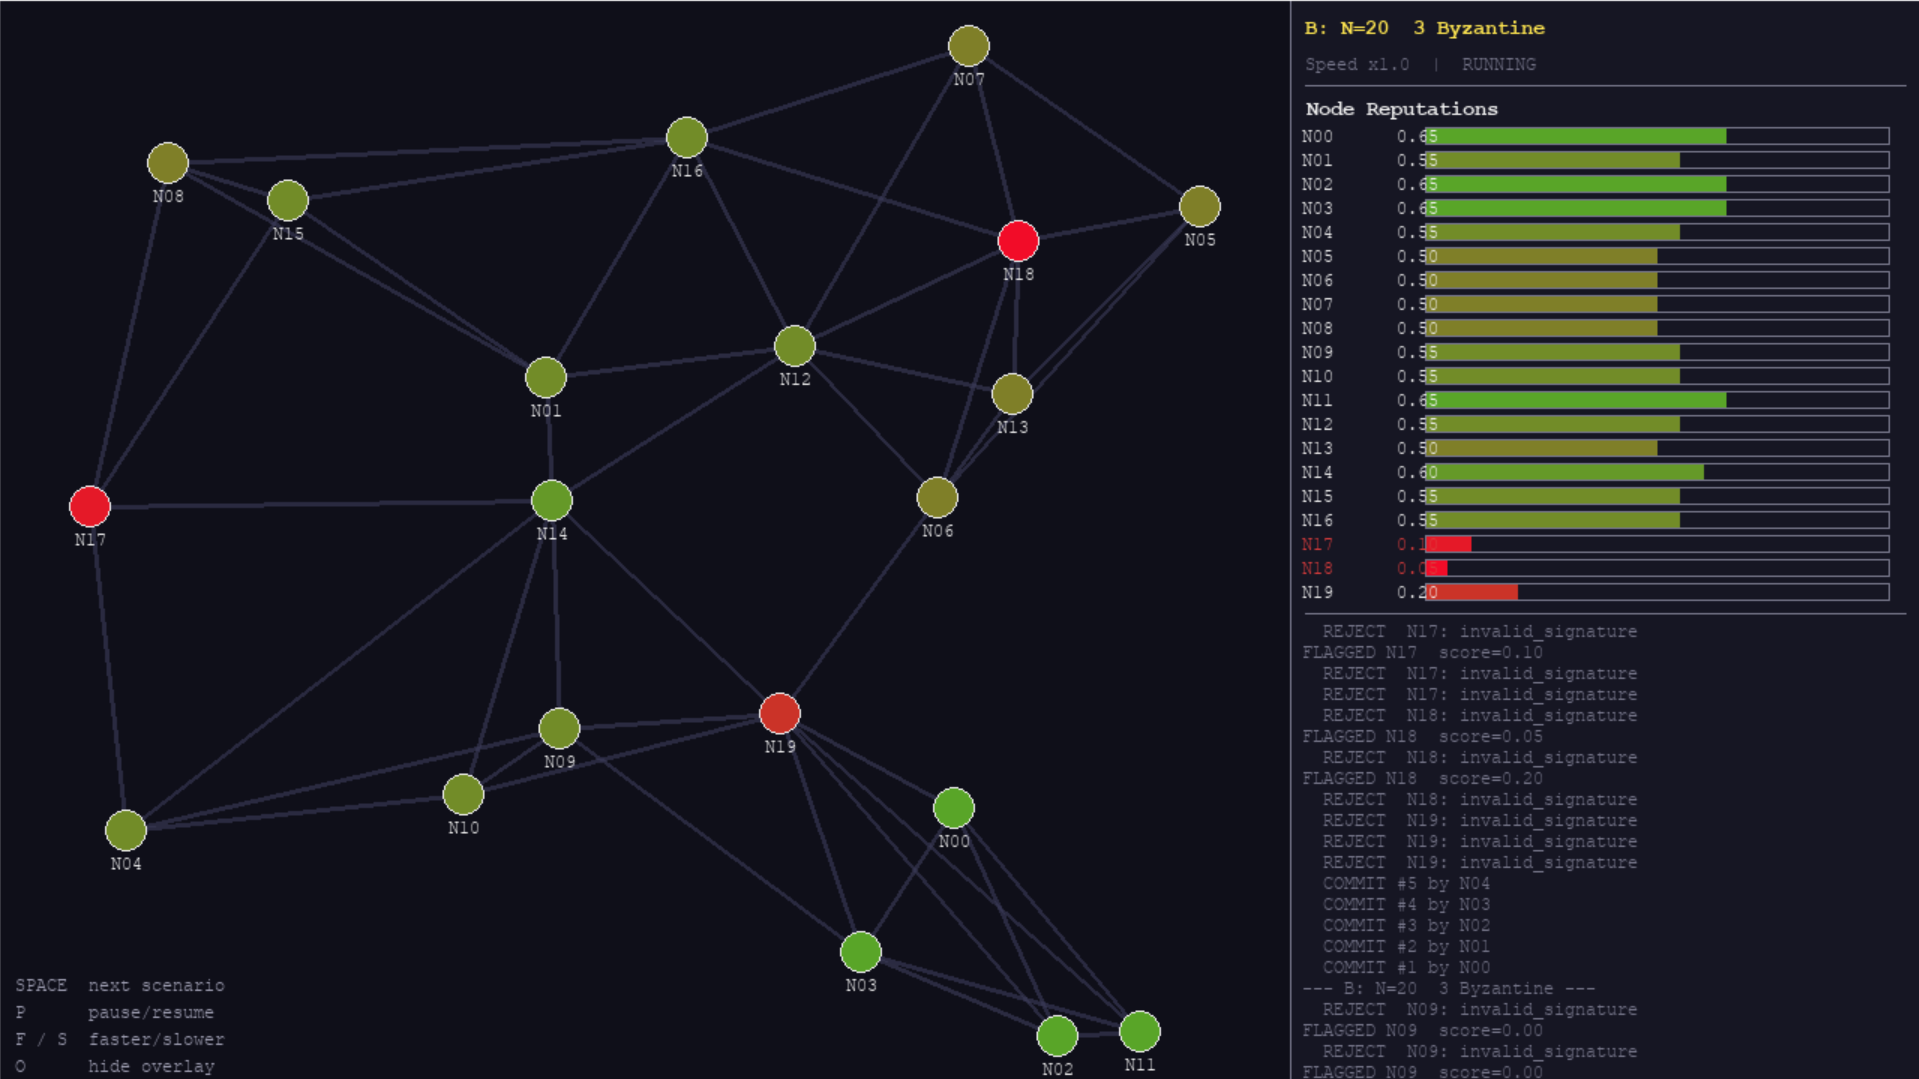
\includegraphics[width=0.8\textwidth]{Figures/hybrid_testbed.png}
	\caption{Hybrid Testbed Architecture: Physical and Virtual Node Integration}
	\label{fig:hybrid_testbed}
\end{figure}

\section{Summary}

This chapter described the design of the decentralized system, focusing on its scalability and security features. The use of a partial mesh, hierarchical FL, and a robust PoA consensus mechanism ensures that the system is suitable for large-scale, infrastructure-independent deployments. The next chapter will detail the implementation of these components.
\chapter{Implementation Details}

This chapter describes the practical implementation of the proposed system, including the firmware for the physical ESP32 nodes and the software environment for the virtual node simulation.

\section{Hardware Implementation: ESP32 Firmware}

The firmware for the physical nodes is developed using the Arduino framework in C++. It manages sensor data acquisition, blockchain operations, and LoRa communication.

\subsection{Cryptographic Implementation}
To ensure security on resource-constrained hardware:
\begin{itemize}
\item \textbf{SHA-256}: Implemented using the mbedTLS library provided by the ESP-IDF.
\item \textbf{ECDSA}: The Micro-ECC library is used for Elliptic Curve Digital Signature Algorithm (P-256 curve) to sign blocks.
\end{itemize}

\subsection{Blockchain Persistence}
The blockchain ledger is persisted in the ESP32's onboard flash memory using the Serial Peripheral Interface Flash File System (SPIFFS). This ensures that the chain state is maintained across device reboots.

\subsection{Sensor Data Acquisition}
Sensors are sampled periodically:
\begin{itemize}
\item \textbf{MPU6050}: Sampled at 100 Hz to detect falls and motion patterns.
\item \textbf{MAX30102}: Interfaced via I2C to obtain PPG signals for HR and SpO2 calculation.
\item \textbf{GPS}: NMEA sentences are parsed to obtain latitude, longitude, and altitude.
\end{itemize}

\section{Simulation Environment: Python Testbed}

The simulation environment is built to exercise the system's logic at scale. It replicates the behavior of the physical nodes in a virtual space.

\subsection{Software Stack}
\begin{itemize}
\item \textbf{Language}: Python 3.9+.
\item \textbf{Numerical Libraries}: \texttt{NumPy} and \texttt{SciPy} for matrix operations and statistical modeling.
\item \textbf{Cryptography}: The \texttt{cryptography} library for ECDSA and SHA-256 operations.
\item \textbf{Visualization}: \texttt{Matplotlib} and \texttt{Seaborn} for generating performance graphs.
\end{itemize}

\subsection{LoRa Physical Layer Modeling}
The simulation uses a log-distance path loss model calibrated to indoor NLOS (Non-Line-of-Sight) measurements:
\[
PL(d) = PL_0 + 10 \cdot n \cdot \log_{10}(d) + X_\sigma
\]
where $PL_0$ is the reference path loss, $n$ is the path loss exponent (3.5), and $X_\sigma$ represents log-normal shadowing with zero mean and standard deviation $\sigma = 8$ dB. This model determines the Packet Delivery Ratio (PDR) between any two nodes.

\section{Federated Learning Implementation}

The Federated Learning layer is implemented as a set of classes in Python, which can be ported to C++ for the ESP32.

\begin{algorithm}[H]
\caption{Federated Averaging with Differential Privacy}
\label{alg:fedavg_dp}
\begin{algorithmic}[1]
\REQUIRE Local weights $w_i$, Privacy parameters $\epsilon, \delta$, Sensitivity $C$
\STATE $\sigma \leftarrow \frac{C}{\epsilon} \sqrt{2 \ln(1.25/\delta)}$ \COMMENT{Calculate noise magnitude}
\STATE $w_i^{noisy} \leftarrow w_i + \mathcal{N}(0, \sigma^2)$ \COMMENT{Add Gaussian noise}
\STATE Broadcast $w_i^{noisy}$ to peers in cluster
\STATE \textbf{On receiving $\{w_j^{noisy}\}$ from peers:}
\STATE $w_{avg} \leftarrow \frac{1}{|K|} \sum_{j \in K} w_j^{noisy}$ \COMMENT{Average received weights}
\STATE Update local model with $w_{avg}$
\end{algorithmic}
\end{algorithm}

\section{Communication Protocol}

The mesh communication is implemented using a custom gossip protocol.

\begin{algorithm}[H]
\caption{Gossip-based Block Propagation}
\label{alg:gossip}
\begin{algorithmic}[1]
\REQUIRE Incoming Block $B$, Fanout $f$, Local Chain $C$
\IF{$Hash(B)$ is in $seen\_cache$}
    \STATE \textbf{Discard} $B$ \COMMENT{Prevent infinite loops}
\ELSE
    \STATE $seen\_cache.add(Hash(B))$
    \IF{PoA\_Validate($B$, $C$) == APPROVE}
        \STATE $C.append(B)$
        \STATE $Peers \leftarrow SelectRandom(f, neighbors)$
        \FORALL{$p \in Peers$}
            \STATE Send $B$ to $p$
        \ENDFOR
    \ENDIF
\ENDIF
\end{algorithmic}
\end{algorithm}

\section{Summary}

The implementation successfully bridges the gap between hardware-constrained execution and large-scale simulation. By using the same cryptographic and consensus logic in both C++ and Python, the hybrid testbed provides a consistent environment for evaluating the system. The next chapter will present the results obtained from this implementation.
\chapter{Results and Analysis}

This chapter presents the results obtained from the simulation of the decentralized LoRa mesh system. The evaluation covers blockchain integrity, consensus performance, Byzantine fault tolerance, and the convergence of the Federated Learning model.

\section{Blockchain Integrity and Tamper Detection}

The core blockchain implementation was tested for its ability to detect data tampering. A single node created 10 blocks, and one block's payload was subsequently modified.

\begin{itemize}
\item \textbf{Result}: The tamper detection mechanism correctly identified the modified block at the exact index where the mutation occurred.
\item \textbf{Inference}: The combination of SHA-256 hashing and ECDSA signatures provides a robust guarantee of data integrity.
\end{itemize}

\section{Consensus Performance (PoA)}

Consensus latency was measured in a 2-node mesh proposing valid and invalid blocks.

\begin{itemize}
\item \textbf{Latency}: The average consensus latency in the simulation was observed between 0.13 ms and 0.19 ms.
\item \textbf{Discussion}: While this latency is low in a simulation environment, it scales with the number of peers. On real hardware, this would be dominated by LoRa transmission times, estimated at 1000-3000 ms per block.
\end{itemize}

\section{Byzantine Fault Tolerance (BFT)}

The system's resilience was tested against 6 different types of attacks, including invalid signatures, tampered payloads, impossible sensor values, and replay attacks.

\begin{table}[htb]
\centering
\caption{Byzantine Attack Rejection Results}
\label{tab:bft_results}
\begin{tabular}{|l|l|l|}
\hline
\textbf{Attack Type} & \textbf{Rejection Point} & \textbf{Result} \\
\hline
Invalid Signature & Check 1 & Rejected \\
Tampered Payload & Check 2 & Rejected \\
Impossible Sensors & Check 5 & Rejected \\
GPS Teleport & Check 5 & Rejected \\
Replay Attack & Check 4 & Rejected \\
Counter Manipulation & Check 4 & Rejected \\
\hline
\end{tabular}
\end{table}

\section{Federated Learning Convergence}

The convergence of the FL model was evaluated using Federated Averaging with Differential Privacy.

\subsection{Privacy-Utility Tradeoff}
The impact of the privacy budget ($\epsilon$) on convergence was analyzed. A lower $\epsilon$ (higher privacy) results in a higher convergence floor due to the added Gaussian noise.

\begin{table}[htb]
\centering
\caption{DP Privacy-Utility Tradeoff}
\label{tab:dp_tradeoff}
\begin{tabular}{|c|c|l|}
\hline
\textbf{Epsilon ($\epsilon$)} & \textbf{Noise Sigma ($\sigma$)} & \textbf{Effect on Convergence} \\
\hline
1.0 & 4.85 & Models diverge; noise dominates signal. \\
10.0 & 0.485 & Convergence floor at $\approx 1.37$ in 10 rounds. \\
50.0 & 0.097 & Clean convergence in $< 5$ rounds. \\
\hline
\end{tabular}
\end{table}

\section{N-Node Scaling and Mesh Performance}

Scaling tests were conducted for 10, 20, and 50 nodes in a $200m \times 200m$ area.

\subsection{LoRa Packet Delivery Ratio (PDR)}
The PDR follows the log-distance path loss model, as shown in Figure \ref{fig:lora_pdr}. The usable range is approximately 110m for 90\% delivery in an indoor NLOS environment.

\begin{figure}[H]
	\centering
	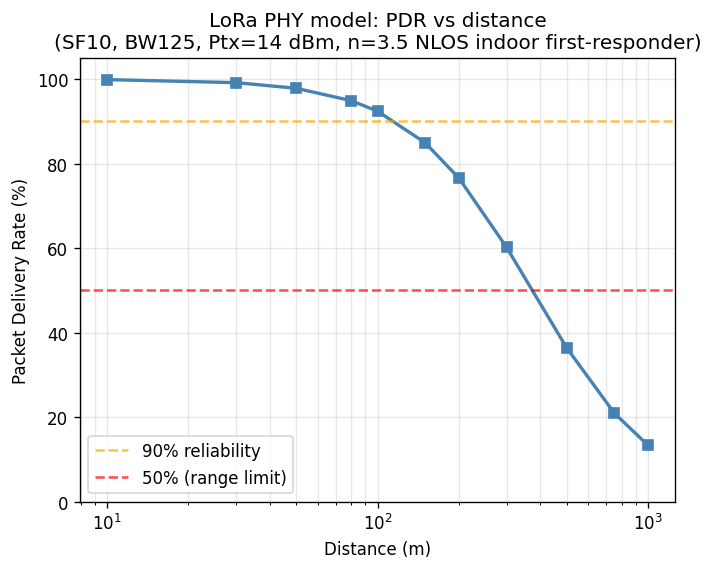
\includegraphics[width=0.8\textwidth]{Figures/lora_pdr_model.png}
	\caption{LoRa PDR vs Distance Model}
	\label{fig:lora_pdr}
\end{figure}

\subsection{Latency and Node Count}
Consensus latency grows sub-linearly with $N$ due to the partial mesh topology ($O(\sqrt{N})$ peers), as illustrated in Figure \ref{fig:latency_vs_n}.

\begin{figure}[H]
	\centering
	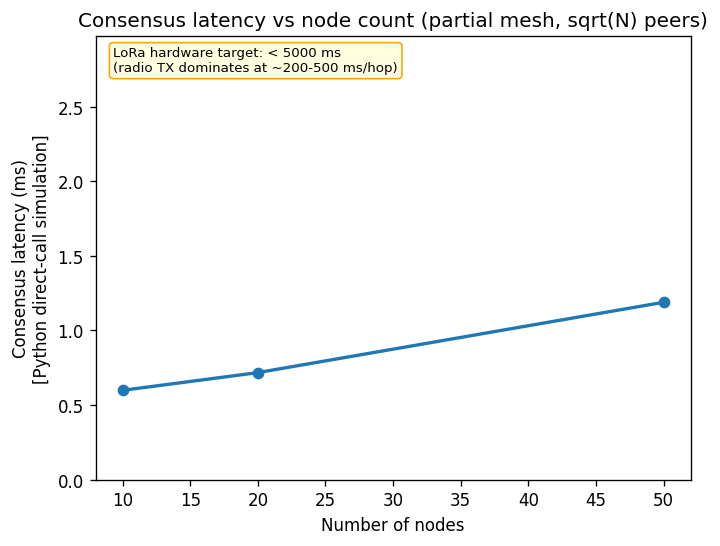
\includegraphics[width=0.8\textwidth]{Figures/latency_vs_n.png}
	\caption{Consensus Latency vs Node Count ($N$)}
	\label{fig:latency_vs_n}
\end{figure}

\subsection{Delivery Rate under Failures}
The gossip protocol maintained an 80\% delivery rate even when 10\% of the nodes simultaneously failed (Figure \ref{fig:delivery_vs_failures}).

\begin{figure}[H]
	\centering
	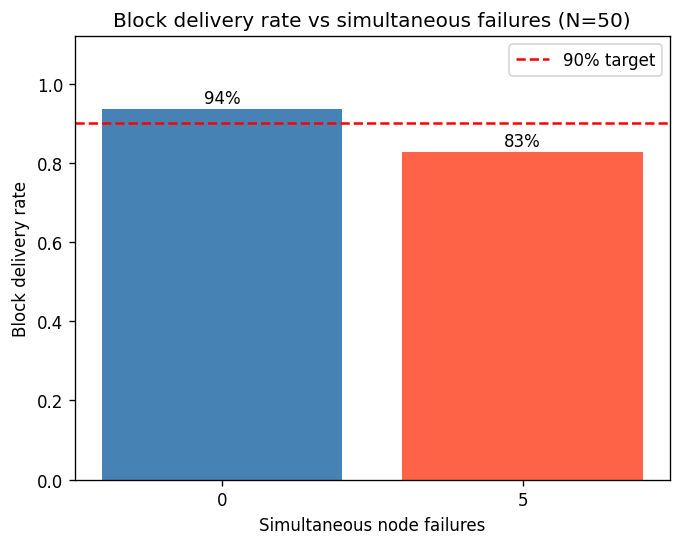
\includegraphics[width=0.8\textwidth]{Figures/delivery_vs_failures.png}
	\caption{Block Delivery Rate vs Number of Failures}
	\label{fig:delivery_vs_failures}
\end{figure}

\subsection{Byzantine Rejection Rate}
The rejection rate for Byzantine attacks was 100\% across different network sizes, as shown in Figure \ref{fig:byz_rejection}.

\begin{figure}[H]
	\centering
	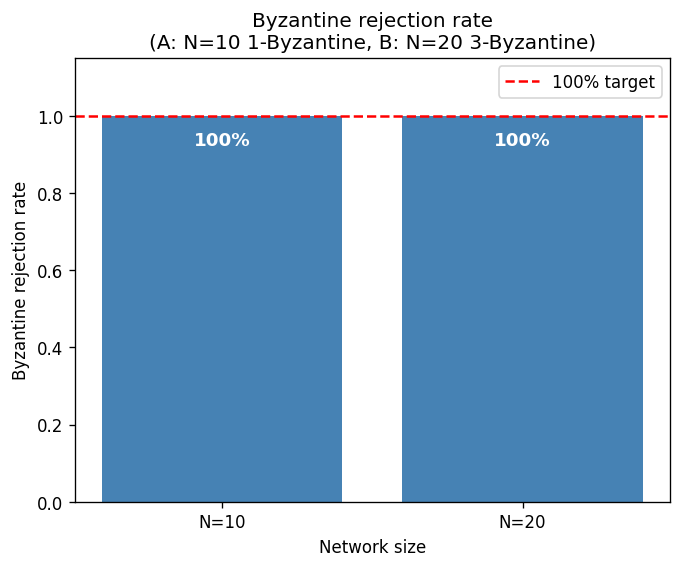
\includegraphics[width=0.8\textwidth]{Figures/byz_rejection_rate.png}
	\caption{Byzantine Attack Rejection Rate}
	\label{fig:byz_rejection}
\end{figure}

\subsection{Flat vs. Hierarchical FL}
Hierarchical FedAvg achieved the same convergence floor as flat FedAvg but with a 5x reduction in global communication overhead at $N=20$ (Figure \ref{fig:fl_convergence}).

\begin{figure}[H]
	\centering
	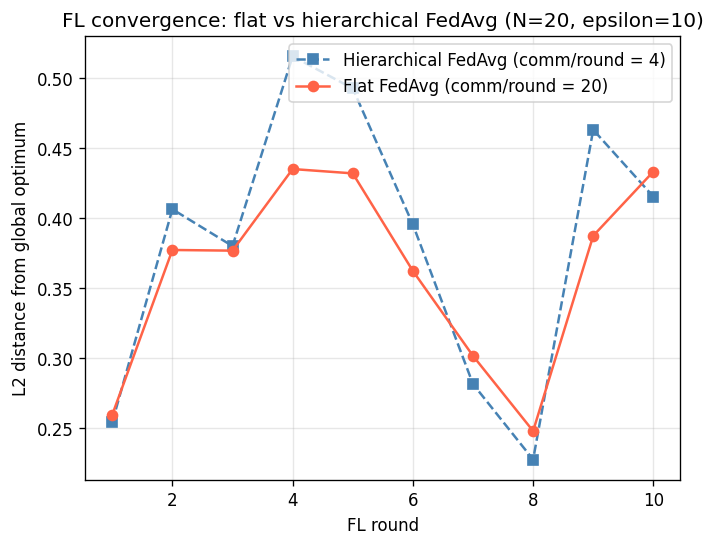
\includegraphics[width=0.8\textwidth]{Figures/fl_convergence.png}
	\caption{FL Convergence: Flat vs. Hierarchical FedAvg}
	\label{fig:fl_convergence}
\end{figure}

\section{Network Partition and Healing}

The system's ability to recover from network partitions was validated.
\begin{itemize}
\item \textbf{Scenario}: 20 nodes split into two groups; Group A commits 3 blocks while Group B is isolated.
\item \textbf{Result}: After reconnection, Group B successfully synced its chain with Group A in $< 1$ ms (simulation time).
\item \textbf{Hardware Estimate}: Total estimated hardware sync time for 2 missed blocks is $\approx 1.5$ seconds.
\end{itemize}

\section{Summary}

The results demonstrate that the proposed system is secure, scalable, and resilient. The PoA consensus effectively isolates Byzantine nodes, and the hierarchical FL approach significantly reduces communication costs without sacrificing accuracy. The next chapter will conclude the report and discuss future work.
\chapter{Conclusion and Future Scope}

The development of a decentralized LoRa mesh system with blockchain and Federated Learning addresses the critical need for secure, infrastructure-independent communication in tactical and disaster response scenarios. This chapter summarizes the project's achievements and outlines potential directions for future research.

\section{Conclusion}

This project successfully designed and simulated a robust monitoring system for first responders. By integrating a lightweight Proof-of-Authority blockchain, the system ensures that all sensor data—including GPS, heart rate, and blood oxygen levels—is recorded in a tamper-proof and cryptographically signed ledger. This provides an immutable audit trail for incident reconstruction and legal accountability.

The implementation of a Frequency-Hopping Spread Spectrum (FHSS) LoRa communication framework ensures resilience against jamming and interference, while the self-organizing mesh topology allows for reliable data propagation without centralized infrastructure. Scalability challenges were addressed through the use of a partial mesh topology and a hierarchical Federated Learning approach, which significantly reduced communication overhead.

The Federated Learning layer enables collective anomaly detection while preserving individual privacy through the use of Differential Privacy. The simulation results validated the system's ability to maintain high delivery rates under node failures, effectively isolate Byzantine nodes, and converge toward an accurate global model despite the addition of privacy-preserving noise.

\section{Future Scope}

While the simulation results are promising, several areas remain for future exploration:
\begin{itemize}
\item \textbf{Hardware-in-the-Loop Testing}: Full-scale deployment on physical ESP32 nodes to validate the timing and power consumption characteristics of the blockchain and FL layers in real-world conditions.
\item \textbf{Realistic Mobility Models}: Integrating pedestrian mobility models (e.g., SUMO) to better simulate the movement patterns of first responders in complex indoor environments.
\item \textbf{Advanced Physiological Modeling}: Using more diverse datasets such as MIMIC-III for heart rate and SpO2 waveforms to improve the accuracy of the anomaly detection model.
\item \textbf{Dynamic Consensus Sets}: Implementing mechanisms to allow nodes to join and leave the validator set dynamically while maintaining security.
\item \textbf{Energy Efficiency}: Further optimizing the cryptographic and communication operations to extend the battery life of the wearable nodes.
\end{itemize}

\section{Learning Outcomes of the Project}

\begin{itemize}
\item Deep understanding of LoRa technology and wireless mesh networking challenges.
\item Implementation of lightweight cryptographic primitives on resource-constrained microcontrollers.
\item Design and validation of Proof-of-Authority consensus mechanisms for private blockchains.
\item Hands-on experience with Federated Learning and Differential Privacy for privacy-preserving AI.
\item Development of hybrid testbeds combining physical hardware with large-scale software simulations.
\item Statistical analysis and visualization of network performance metrics using Python.
\end{itemize}

\appendix
\chapter{Code}

\section{Dataset Generation using XTTS-v2}

The following Python script was used for generating the speech dataset using the XTTS-v2 multilingual text-to-speech model. The implementation mounts Google Drive, loads reference speaker audio samples, synthesizes speech samples from text prompts, and stores the generated dataset for further processing.

\begin{tcblisting}{listing only,colback=gray!10!white, breakable, boxsep=0pt,top=1mm,bottom=1mm,left=1mm,right=1mm,
listing options={
language=Python,
basicstyle=\small\ttfamily,
keywordstyle=\color{blue},
commentstyle=\color{gray},
backgroundcolor=\color{gray!25},
escapechar=!}}

from google.colab import drive
import os
import torch
from TTS.api import TTS
from tqdm.notebook import tqdm

# Mount Google Drive
drive.mount('/content/drive', force_remount=True)

DRIVE_BASE = "/content/drive/MyDrive"
INPUT_FOLDER = os.path.join(DRIVE_BASE, "sample")
TEXT_FILE_PATH = "/content/text.txt"
OUTPUT_BASE = os.path.join(DRIVE_BASE, "output")

os.makedirs(OUTPUT_BASE, exist_ok=True)

# Select GPU if available
device = "cuda" if torch.cuda.is_available() else "cpu"
print(f"Running on: {device}")

# Load XTTS-v2 model
tts = TTS(
    model_name="tts_models/multilingual/multi-dataset/xtts_v2",
    gpu=(device == "cuda")
).to(device)

# Read text samples
with open(TEXT_FILE_PATH, "r", encoding="utf-8") as f:
    all_lines = [
        line.strip().strip("'").strip('"')
        for line in f.readlines()
    ][:1000]

# Process male speaker samples
gender_targets = ['m']

for gender in gender_targets:

    gender_path = os.path.join(INPUT_FOLDER, gender)

    speaker_files = sorted([
        f for f in os.listdir(gender_path)
        if f.lower().endswith('.wav')
    ])

    for wav_file in speaker_files:

        ref_wav = os.path.join(gender_path, wav_file)
        speaker_name = os.path.splitext(wav_file)[0]

        speaker_out_dir = os.path.join(
            OUTPUT_BASE,
            gender,
            speaker_name
        )

        os.makedirs(speaker_out_dir, exist_ok=True)

        pbar = tqdm(
            total=len(all_lines),
            desc=f"Generating {speaker_name}",
            unit="line"
        )

        for idx, text in enumerate(all_lines):

            if not text:
                pbar.update(1)
                continue

            output_path = os.path.join(
                speaker_out_dir,
                f"{idx}.wav"
            )

            if os.path.exists(output_path):
                pbar.update(1)
                continue

            try:
                tts.tts_to_file(
                    text=text,
                    speaker_wav=ref_wav,
                    file_path=output_path,
                    language="en"
                )

            except Exception as e:
                print(f"Error at line {idx}: {e}")

            pbar.update(1)

        pbar.close()

print("Dataset generation completed successfully.")

\end{tcblisting}

\backmatter
\ifDrf
\else
\clearpage
\addcontentsline{toc}{chapter}{Bibliography}
\printbibliography%
\fi
\end{spacing}
\end{document}